\documentclass{article}

\usepackage{arxiv}

\usepackage[utf8]{inputenc}
\usepackage[T1]{fontenc}
\usepackage{hyperref}
\usepackage{url}
\usepackage{booktabs}
\usepackage{amsfonts}
\usepackage{amsmath}
\usepackage{nicefrac}
\usepackage{microtype}
\usepackage{graphicx}
\graphicspath{ {../assets/} }

\title{Does Where You Distill Matter? An Exploratory Study of\\
Position-Selective Token Distillation for Reasoning Models}

\author{
  Astarag Mohapatra \\
  \texttt{astarag2843@gmail.com} \\
}

\begin{document}
\maketitle

\begin{abstract}
Knowledge distillation for large reasoning models typically applies a uniform loss over every generated token.
In this paper, we ask a simple question: does the \emph{position} of a token within a reasoning chain affect how useful it is as a distillation target?
We build on On-Policy Self-Distillation (OPSD)~\cite{opsd2025}, which trains a student model by minimizing a forward KL divergence against a fixed teacher, and introduce six position-selective variants that restrict distillation to tokens drawn from the first, middle, or last sentence of each reasoning paragraph, with top-$k$ selection ($k\in\{1,2\}$).
To motivate this, we run a Mann-Whitney U test on per-token KL proxy values and find that sentence-start tokens exhibit significantly higher variance than middle or end tokens, suggesting they carry richer gradient signal.
Our preliminary experiments on Qwen3-1.7B across AIME24, AIME25, and HMMT25 show mixed but occasionally promising results: \texttt{firstsent\_topk2} reaches 40.0\% Avg@8 on AIME25 at step 75, and \texttt{lastsent\_topk2} peaks at 60.8\% MajVote@8 on AIME24 at step 75, compared to the full-token OPSD baseline of 37.5\% and 52.5\% respectively at that step.
These gains are not stable across all checkpoints and benchmarks, and training curves are noisy — we do not claim a definitive improvement.
Rather, we offer this as a useful datapoint: a sparser distillation signal concentrated at structurally motivated positions can sometimes match or briefly exceed full-token distillation, which motivates further investigation.
\end{abstract}

\section{Introduction}

\begin{quote}
\textit{``The scariest moment is always just before you start. After that, things can only get better.''}\\
\hfill --- Stephen King
\end{quote}

Training reasoning models is expensive.
Methods like GRPO~\cite{shao2024deepseekmath} and self-distillation~\cite{opsd2025} have shown that a student model can be improved by learning from a stronger (or fixed) teacher's output distribution over long chain-of-thought completions.
However, most of these methods apply the distillation loss uniformly across every token in the generated sequence — including filler words, punctuation, and repetitive connectives that likely carry little information.

Recent work has shown that this uniformity is not necessary.
Wang et al.~\cite{wang2026beyond} find that roughly 20\% of tokens — those with the highest entropy under the model's distribution — account for the vast majority of learning signal in reinforcement learning for reasoning.
These high-entropy ``minority tokens'' are the decision points: the places where the model is genuinely uncertain, and where getting the prediction right or wrong has the most downstream consequence.
This motivates a natural design choice in distillation: focus the training signal on high-entropy tokens and ignore the rest.

The question we explore in this paper is a step further: \emph{where do these high-entropy tokens tend to appear in a reasoning chain?}
In long-form mathematical reasoning, a model's output is structured into paragraphs — each paragraph represents a coherent sub-step or shift in reasoning strategy, and a new paragraph begins when the model transitions to a new line of thought.
These paragraph boundaries are natural candidates for high-entropy positions: the model must decide not just what word comes next, but what direction to take the reasoning.
Within a paragraph, we similarly expect the first sentence to carry more uncertainty than the middle or the end, which tend to elaborate on an already-committed direction.

We test this hypothesis empirically.
Using a per-token KL proxy, we find that sentence-start tokens have significantly higher variance than middle or end tokens (Section~\ref{sec:motivation}).
We then introduce six position-selective distillation variants on top of OPSD and evaluate them on three mathematical reasoning benchmarks (Section~\ref{sec:experiments}).

Our contributions are:
\begin{itemize}
    \item A positional entropy analysis showing that sentence-start tokens have significantly higher KL proxy variance than middle or end tokens (Section~\ref{sec:motivation}).
    \item Six position-selective distillation variants that restrict training signal to specific sentence positions within paragraphs (Section~\ref{sec:method}).
    \item Preliminary experimental results on three math benchmarks, with an honest discussion of what works, what does not, and why the results are inconclusive (Section~\ref{sec:results}).
\end{itemize}

\section{Background}
\label{sec:background}

\paragraph{On-Policy Self-Distillation (OPSD).}
OPSD~\cite{opsd2025} trains a student model on reasoning traces sampled from itself (on-policy), using a fixed copy of the model as the teacher.
The training objective minimizes a clipped forward KL divergence between the teacher's token-level distribution $p_{\text{teacher}}$ and the student's $p_{\text{student}}$:
\begin{equation}
    \mathcal{L}_{\text{OPSD}} = \sum_{t} \text{clip}\!\left(\log p_{\text{teacher}}(x_t) - \log p_{\text{student}}(x_t),\; -c,\; c\right)
\end{equation}
where $c$ is a clipping threshold (set to $0.05$ in our experiments).
The student is a LoRA adapter~\cite{hu2022lora} on top of a pretrained base model, and the teacher is a frozen copy of the initial model.
Training data comes from OpenThoughts~\cite{openthoughts2025}, a dataset of long-form mathematical reasoning traces.

\paragraph{Selective distillation.}
Prior work on knowledge distillation has explored selecting which tokens or layers to distill.
Methods like MiniLLM~\cite{gu2024minillm} and DistiLLM~\cite{ko2024distillm} focus on reverse KL or sequence-level objectives.
Token-level selection has been explored in the context of top-$k$ vocabulary distillation~\cite{shi2024mini}, but positional selection within generated reasoning chains has received less attention.

\section{Motivation: Positional Entropy Analysis}
\label{sec:motivation}

Before designing position-selective variants, we ask whether different sentence positions in a reasoning paragraph have measurably different distillation signal.
We use the per-token KL proxy $\log p_{\text{teacher}} - \log p_{\text{student}}$ as a proxy for how much each token contributes to the distillation loss.

We classify each token in a set of OpenThoughts reasoning traces by its sentence position within its paragraph: \emph{first sentence}, \emph{middle sentence}, \emph{last sentence}, or \emph{single-sentence paragraph}.
Table~\ref{tab:kl_stats} reports the mean and standard deviation of this proxy, along with 95\% confidence intervals.

\begin{table}[h]
\caption{Per-token KL proxy ($\log p_{\text{teacher}} - \log p_{\text{student}}$) by sentence position.}
\label{tab:kl_stats}
\centering
\begin{tabular}{lrrrr}
\toprule
Position & Mean & Std & 95\% CI & $n$ \\
\midrule
Start  & $-0.166$ & $1.617$ & $[-0.185,\,-0.147]$ & 28{,}344 \\
Middle & $-0.074$ & $0.493$ & $[-0.084,\,-0.065]$ & 10{,}174 \\
End    & $-0.102$ & $0.569$ & $[-0.110,\,-0.095]$ & 24{,}079 \\
Single & $-0.116$ & $1.206$ & $[-0.119,\,-0.112]$ & 456{,}489 \\
\bottomrule
\end{tabular}
\end{table}

The start position has notably higher standard deviation ($1.617$) compared to middle ($0.493$) and end ($0.569$), indicating that sentence-start tokens are more spread out in terms of how much the teacher and student disagree.
We run one-sided Mann-Whitney U tests to check whether start tokens have higher KL proxy values than other positions:

\begin{table}[h]
\caption{One-sided Mann-Whitney U test results (row $>$ column).}
\label{tab:mwu}
\centering
\begin{tabular}{lll}
\toprule
Comparison & $p$-value & Interpretation \\
\midrule
Start $>$ Middle & $1.00$ & n.s. — start has higher variance, not higher mean \\
Start $>$ End    & $2.31 \times 10^{-20}$ & significant \\
Middle $>$ End   & $9.79 \times 10^{-36}$ & significant \\
\bottomrule
\end{tabular}
\end{table}

While the means are all negative (student slightly overconfident relative to teacher), the variance at the start position is much larger, meaning the signal is more extreme in both directions.
We hypothesize that these high-variance tokens — often the first substantive word of a new sentence — represent decision points where the student's predictions diverge most from the teacher, making them more informative training targets.

\section{Method: Position-Selective Token Distillation}
\label{sec:method}

\paragraph{Paragraph and sentence segmentation.}
We segment each generated reasoning trace into paragraphs by splitting on blank lines.
Within each paragraph, we identify sentences using punctuation-based heuristics.
For a paragraph with $S$ sentences, we label sentence $1$ as \emph{first}, sentence $S$ as \emph{last}, and sentences $2, \ldots, S-1$ as \emph{middle}.
A paragraph with a single sentence is treated as both first and last.

\paragraph{Token selection.}
Within each selected sentence, we apply top-$k$ selection: we pick the $k$ tokens with the highest absolute KL proxy value within that sentence as the distillation targets.
All other tokens receive zero loss weight.

We test the following six variants, plus the full-token OPSD baseline:
\begin{enumerate}
    \item \textbf{firstsent\_topk1}: top-1 token from the first sentence of each paragraph
    \item \textbf{middlesent\_topk1}: top-1 token from the middle sentence
    \item \textbf{lastsent\_topk1}: top-1 token from the last sentence
    \item \textbf{firstsent\_topk2}: top-2 tokens from the first sentence
    \item \textbf{lastsent\_topk2}: top-2 tokens from the last sentence
    \item \textbf{parafirsttok\_topk1}: the single first token of each paragraph (no sentence parsing)
\end{enumerate}

We also attempted \textbf{middlesent\_topk2} but found that training diverged, so we exclude it from the results.

\section{Experiments}
\label{sec:experiments}

\paragraph{Setup.}
We fine-tune Qwen3-1.7B~\cite{qwen3} using LoRA ($r=64$, $\alpha=128$, applied to all projection matrices) on OpenThoughts data.
Training uses AdamW with learning rate $5\times10^{-6}$, gradient clipping at $0.1$, temperature $1.1$, top-$p=0.95$, top-$k=20$, and $\beta=0$ (no KL penalty on the policy).
The teacher is a fixed copy of the initial model.
We train for 100 steps and evaluate checkpoints at steps 25, 50, 75, and 100.

\paragraph{Evaluation.}
We evaluate on three mathematical reasoning benchmarks: AIME 2024 (AIME24), AIME 2025 (AIME25), and HMMT 2025 (HMMT25).
Inference uses vLLM with thinking mode enabled, temperature $1.0$, top-$p=0.95$, top-$k$ disabled, min-$p=0.0$, presence penalty $0.0$, and a maximum of $38{,}912$ new tokens.
We draw $n=8$ samples per problem and report three metrics: \textbf{Pass@8} (fraction of problems solved by at least one sample), \textbf{MajVote@8} (majority-vote accuracy over 8 samples), and \textbf{Avg@8} (mean per-sample accuracy).

\paragraph{Active loss tokens.}
Figure~\ref{fig:active_tokens} shows the number of active loss tokens per step for each variant.
The full-token OPSD baseline uses roughly 3{,}000--3{,}500 tokens per update, while all positional variants use far fewer — often under 200 for top-1 sentence variants and around 300 for top-2 variants.
This confirms that position-selective distillation is genuinely sparse compared to the baseline.

\begin{figure}[ht]
    \centering
    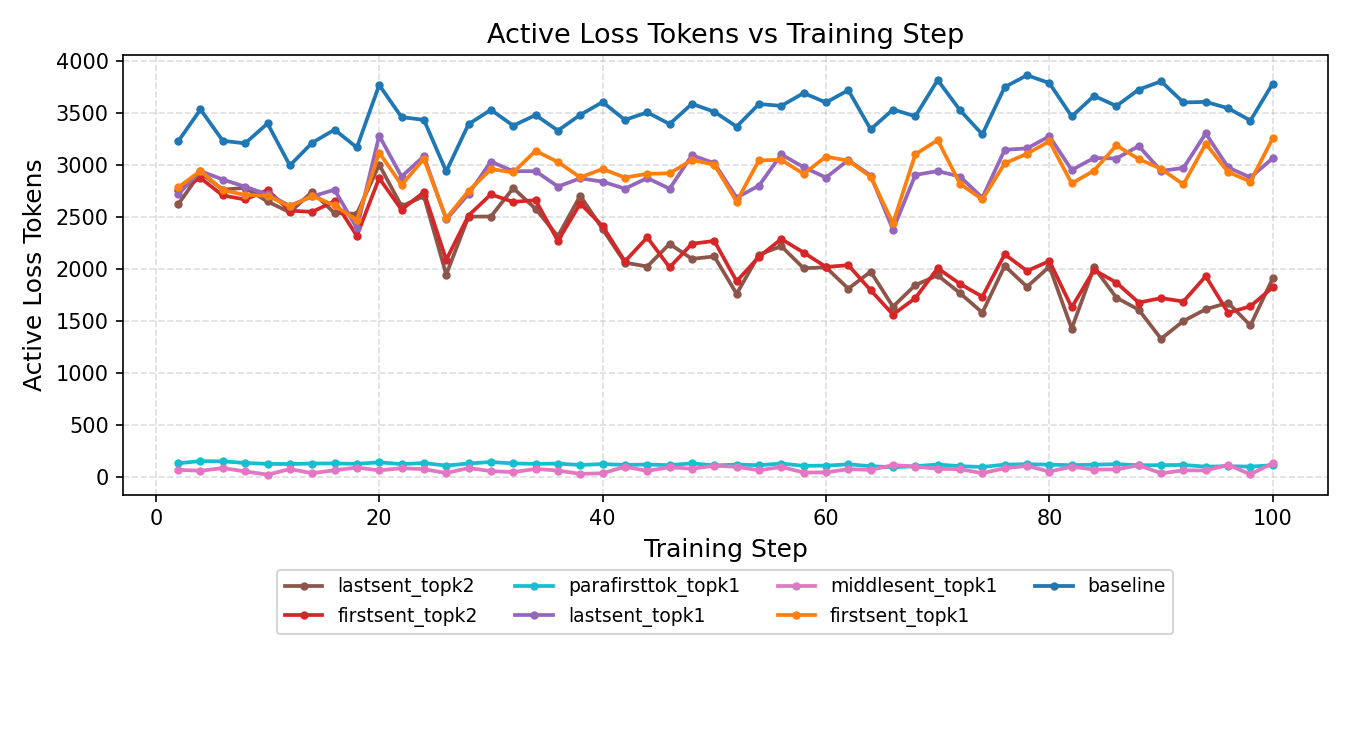
\includegraphics[width=\textwidth]{plot_active_tokens.png}
    \caption{Active loss tokens per training step for each variant. The baseline (full-token OPSD) uses far more tokens per update than any positional variant, confirming the sparsity of the position-selective approach.}
    \label{fig:active_tokens}
\end{figure}

\paragraph{Benchmark results.}
Figures~\ref{fig:avg8}, \ref{fig:majvote8}, and \ref{fig:pass8} show all metrics across training steps for all variants.

\begin{figure}[h]
    \centering
    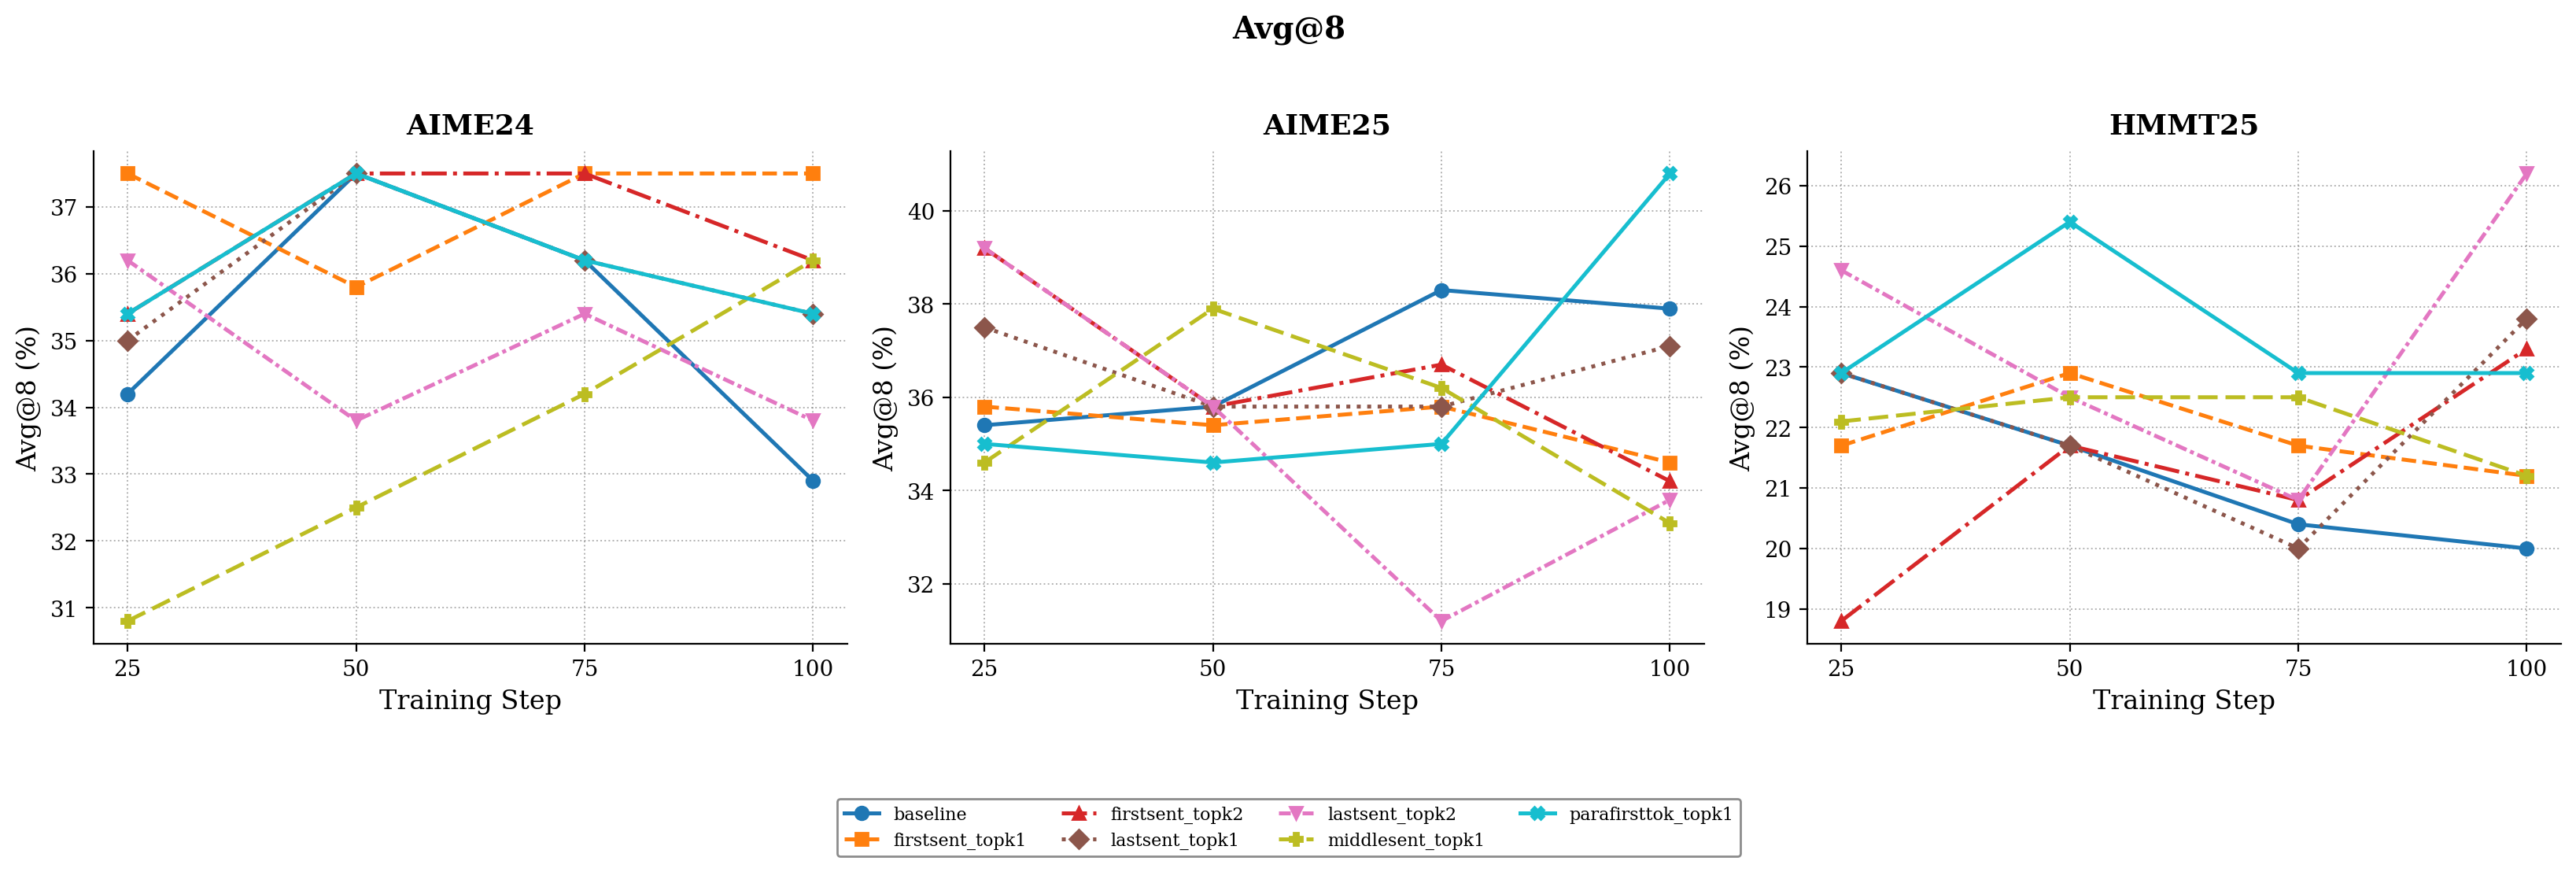
\includegraphics[width=\textwidth]{plot_Avgat8.png}
    \caption{Avg@8 across training steps on AIME24, AIME25, and HMMT25.}
    \label{fig:avg8}
\end{figure}

\begin{figure}[h]
    \centering
    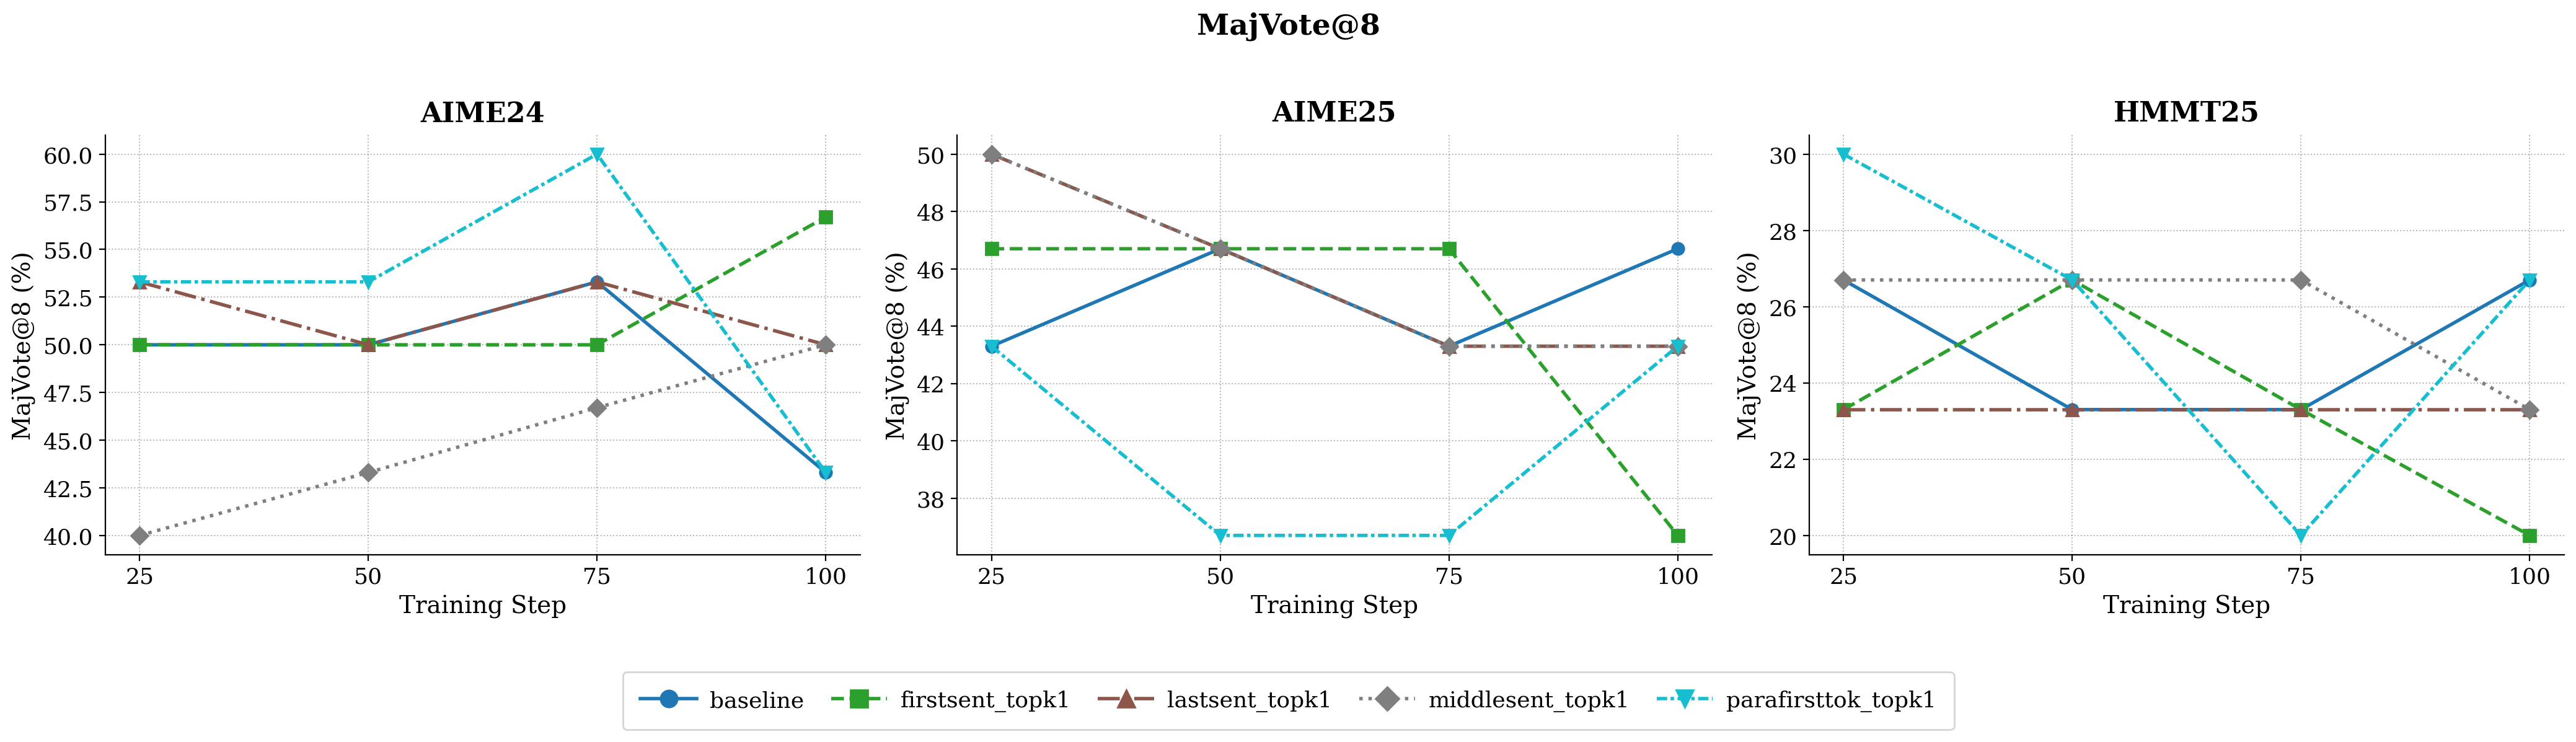
\includegraphics[width=\textwidth]{plot_MajVoteat8.png}
    \caption{MajVote@8 across training steps on AIME24, AIME25, and HMMT25.}
    \label{fig:majvote8}
\end{figure}

\begin{figure}[h]
    \centering
    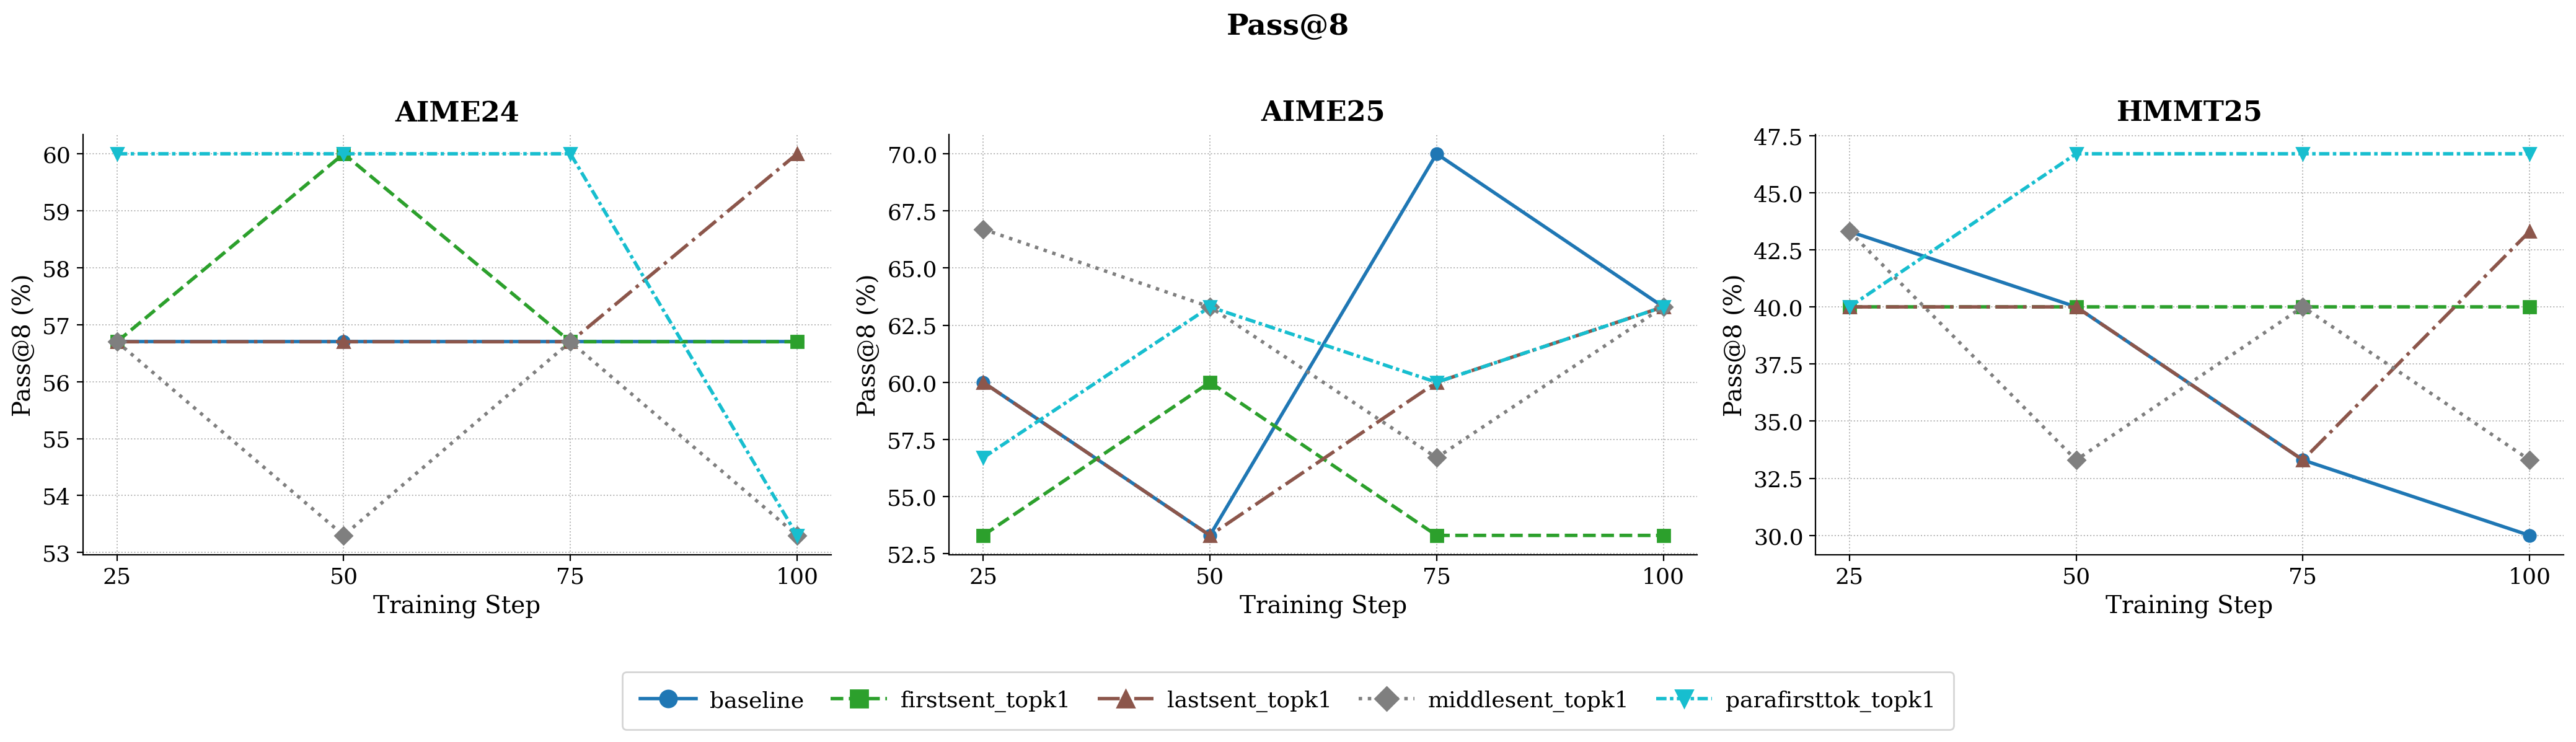
\includegraphics[width=\textwidth]{plot_Passat8.png}
    \caption{Pass@8 across training steps on AIME24, AIME25, and HMMT25.}
    \label{fig:pass8}
\end{figure}

\section{Results and Discussion}
\label{sec:results}

The honest summary is that results are noisy and no single variant consistently outperforms the full-token OPSD baseline across all benchmarks and metrics.
However, a few patterns are worth noting.

\textbf{First and last sentence variants occasionally match the baseline.}
\texttt{firstsent\_topk2} and \texttt{lastsent\_topk2} occasionally match or slightly exceed the baseline on AIME24 and AIME25 at certain checkpoints.
This is notable because these variants use substantially fewer distillation tokens, so they are achieving similar performance with a sparser training signal.

\textbf{Middle sentence underperforms.}
\texttt{middlesent\_topk1} is generally the weakest variant across all three benchmarks, which is consistent with the lower-entropy observation in Section~\ref{sec:motivation} — middle-sentence tokens have the lowest KL proxy variance and may carry the least informative signal.

\textbf{Paragraph-first token is inconsistent.}
\texttt{parafirsttok\_topk1} shows variable behavior across benchmarks and does not clearly align with either the high-entropy or low-entropy story, possibly because the first token of a paragraph is often a formatting token rather than a semantically meaningful decision point.

\textbf{Training curves are unstable.}
All variants show significant fluctuation across the four checkpoints, which makes it difficult to draw firm conclusions from only 100 training steps.
A longer run with more checkpoints and multiple seeds would be needed to say anything definitive.

\textbf{Limitations.}
This is a small exploratory study.
We only train one model size (1.7B parameters), run for 100 steps without a hyperparameter search, and evaluate on a narrow set of math benchmarks.
The token selection heuristic (top-$k$ by KL proxy within a sentence) is simple and may not be the best way to identify high-signal tokens.
We also did not explore combining positions (e.g., first and last sentence together).

\section{Conclusion}

We asked whether the position of tokens in a reasoning chain affects their value as distillation targets.
The entropy analysis in Section~\ref{sec:motivation} provides a principled reason to suspect that sentence-start tokens are more informative, and the preliminary results in Section~\ref{sec:results} do not contradict this — but they are also far from conclusive.

The most interesting observation is that sparse, position-selective distillation can sometimes match full-token distillation.
If this holds up in longer training runs, it would suggest that most of the tokens in a reasoning chain contribute little to the distillation objective, and that a smarter selection strategy could substantially reduce the computational cost of distillation.

We see this paper as a small step toward understanding which parts of a reasoning chain matter most for training.
Future work should explore longer training, multiple seeds, larger model sizes, adaptive position selection, and combinations of positions.

\bibliographystyle{unsrt}
\begin{thebibliography}{9}

\bibitem{opsd2025}
Siyan Zhao, Zhuohan Xie, Mengdi Liu, Jiatao Gu, Guo Pang, Fei Chen, and Aditya Grover.
\newblock Self-Distilled Reasoner: On-Policy Self-Distillation for Large Language Models.
\newblock {\em arXiv preprint arXiv:2601.18734}, 2026.

\bibitem{shao2024deepseekmath}
Zhihong Shao, Peiyi Wang, Qihao Zhu, Runxin Xu, Junxiao Song, Mingchuan Zhang, Y.~K. Li, Y.~Wu, and Daya Guo.
\newblock DeepSeekMath: Pushing the limits of mathematical reasoning in open language models.
\newblock {\em arXiv preprint arXiv:2402.03300}, 2024.

\bibitem{hu2022lora}
Edward~J. Hu, Yelong Shen, Phillip Wallis, Zeyuan Allen-Zhu, Yuanzhi Li, Shean Wang, Lu~Wang, and Weizhu Chen.
\newblock LoRA: Low-rank adaptation of large language models.
\newblock In {\em ICLR}, 2022.

\bibitem{openthoughts2025}
OpenThoughts Team.
\newblock OpenThoughts: A dataset of long-form reasoning traces.
\newblock \url{https://huggingface.co/datasets/open-thoughts/OpenThoughts-114k}, 2025.

\bibitem{gu2024minillm}
Yuxian Gu, Li~Dong, Furu Wei, and Minlie Huang.
\newblock MiniLLM: Knowledge distillation of large language models.
\newblock In {\em ICLR}, 2024.

\bibitem{ko2024distillm}
Jongwoo Ko, Sungnyun Kim, Tianyi Chen, and Se-Young Yun.
\newblock DistiLLM: Towards streamlined distillation for large language models.
\newblock In {\em ICML}, 2024.

\bibitem{shi2024mini}
Zhenyu Shi, Xuanyu Zhang, Zhen Qin, Shentao Yang, and others.
\newblock Efficient knowledge distillation via token-level vocabulary reduction.
\newblock {\em arXiv preprint}, 2024.

\bibitem{wang2026beyond}
Shuo Wang, Longyue Yu, Chenyang Gao, Ce~Zheng, Siyuan Liu, Renliang Lu, et~al.
\newblock Beyond the 80/20 rule: High-entropy minority tokens drive effective reinforcement learning for LLM reasoning.
\newblock In {\em Advances in Neural Information Processing Systems}, volume~38, pages 115452--115486, 2026.

\bibitem{qwen3}
Qwen Team.
\newblock Qwen3 technical report.
\newblock \url{https://huggingface.co/Qwen/Qwen3-1.7B}, 2025.

\end{thebibliography}

\end{document}
